\section{Evaluation}
\label{sec:evaluation}
In order to evaluate the efficacy of our approach, we examine the overall accuracy of the system in detecting doorway events, as well as the direction of the person's movement.
We investigate the systems robustness to multiple human factors, such as height, walking speed, and clothing / hair color.
We also evaluate the \sysname on two doorways with different lighting settings.
We conducted a study, involving human test subjects, to verify the efficacy of our approach.\footnote{This study was approved by our Institutional Review Board.}
Our experiments are conducted with the \sysname prototype described in \secref{sec:implementation}, with 12 test subjects and 124 individual doorway events.



\begin{table*}[t]
	\begin{tabular}{@{}p{0.8in}p{0.8in}p{1.8in}p{1.0in}p{0.7in}p{0.7in}@{}}
	\toprule
	\multirow{2}{*}{\textbf{Subject}}	&	\multirow{2}{*}{\textbf{Height}} & \multirow{2}{*}{\textbf{Hair/Clothes}} & \multirow{2}{*}{\textbf{Light (Lux)}} & \multicolumn{2}{c}{\textbf{Detected Direction}} 		\\
	& & & & In (\%) & Out (\%) \\\midrule
	1 & 6'1" & Black/Orange & 75 & 100\% & 100\% \\
	2 & 6'1" & Bald/Lt. Blue & 74 & 100\% & 100\% \\
	3 & 5'11" & Brown/Green & 70 & 100\% & 100\% \\
	4 & 5'6" & Pink/Black & 75 & 100\% & 100\% \\
	5 & 6'0" & Brown/Black & 71 & 100\% & 100\% \\
	6 & 6'0" & Tan/Black & 73 & 100\% & 100\% \\
	7 & 6'1" & Brown/Orange & 72 & 100\% & 100\% \\
	8 & 5'10" & Black/Grey & 70 & 100\% & 100\% \\
	9 & 5'3" & Brown/Lt. Blue & 70 & 100\% & 100\% \\
	10 & 6'0" & Bald/Blue & 70 & 100\% & 100\% \\
	\bottomrule
	\end{tabular}
	\caption{Results from 10 test subjects with variable heights, walking speed, hair color, and clothing, walking through a doorway with even artificial lighting on entrance and exit over a reflective floor in the late afternoon. These results show that a \textbf{tuned}, well-lit \sysname occupancy monitor is very accurate at detecting doorway events and direction. \label{tab:detection}}
\end{table*}


\subsection{Methodology and Claims}
The following experiments attempt to address the goals defined in \secref{sec:system}.
We address system availability~(Goal~1) by demonstrating the low power draw of the system itself, and the percent of time it caught doorway events (and the number of doorway events missed) for each doorway test.
% the minimum light intensity at which \sysname can sustain operation and detect doorway events.
We explore variable lighting conditions~(Goal~2) by testing the device under two different lighting conditions.
We address variable human characteristics~(Goal~3) to a large extent by evaluating different walking speeds and the effect of different clothing and hair color on detection patterns.
We claim that ~(Goal~4), concerning form factor, is addressed by our prototype and slim mechanical design, described in \secref{sec:implementation}.
We note that these experiments are best effort, and cannot hope to cover all variability and confounding factors of tracking of diverse persons and buildings.

To process and enable data collection  in our experiments, we gather all electrical signal measurements, except where specified otherwise, using the Saleae Logic~16 logic analyzer\footnote{https://www.saleae.com}, at a sampling rate of 5KS/s and a recording duration of ten (10) seconds.
The analyzer has high impedance ADC's allowing for unobtrusive monitoring of all signals.
This sampling rate is slow, but sufficient to determine the detection events on the doorway, as we are measuring human recognizable events. 
We manually recorded the direction of each doorway event as ground truth to verify the accuracy of \sysname in event detection, compared with the results measured by the logic analyzer.

%%only if time allows:
%%%passing vs. normal entering and exiting of the room
%%%what multiple people entering in close succession looks like to the system and can the system tell the difference between the systems.

%Notes on current testing plan environment:
%tile floor, semi reflective
%door open
%lights on on both sides of the door
%16 solar panels that are alternatively tilted by 10 degrees in either direction (8 panels on each side)
%walking at normal speed through the center of the doorway

%In order to test how well \sysname fares in terms of the availability goal, we tried turning down the light levels till \sysname stopped sustaining operation. Our aim in performing this experiment is to find a threshold above which \sysname sustains operation and is available for detecting ephemeral doorway events as they occur.
%We found that \sysname stops sustaining operation below XXYYZZ lux. This is an acceptable threshold as the average light levels in office environments will be greater than or equal to \SI{70}{\lux}. Even when the light levels fall significantly lower till \SI{40}{\lux}, we are able to detect events but it does affect our direction detection, as outlined in the next section.

\subsection{Detection Accuracy}
This section seeks to understand how well \sysname can perform occupancy monitoring.
We define occupancy monitoring in this context very narrowly; detecting doorway events caused by people walking under \sysname, and further detecting the direction of these people using solar energy harvesting traces. 
In this experiment, we affixed the \sysname prototype to the doorjamb of a reasonably well lit (inside and out) doorway.
This doorway was lit with existing fluorescent  office lighting on both sides, with minimal amounts of natural light from windows.
The door was kept open all through the experiments and the flooring was light colored tiles.
This doorway had nearly equal amounts of light (measured in lux) on both sides.

We had ten (10) participants walk through the doorway at different speeds. 
Each participant walked in and out of the room six times in each direction. 
We evaluated results at three different walking speeds (normal, fast, and slow). 
In order to calculate the speed of each participant, we marked a fixed length path through the door and recorded the time they took to cover it. 
Results indicated average speeds for all participants as follows:  3.7 foot per second (1.12 m/s) for normal, 2.6 foot per second (0.79 m/s) for slow, and 5.36 foot per second (1.6 m/s) fast. 
Furthermore, participants wore different colored clothing (ranging from light to dark) and had different heights that ranged from 5ft 3in (1.6m) to 6ft 1in (1.85m). 
We also considered the hairstyle or headgear of the participants as a factor in the recruitment process.

\noindpar{Results:}
The results of this experiment are shown in \tabref{tab:detection}.
We list the height, hair / hat color, and light levels alongside detection. 
\sysname was very successful in detecting both doorway events, and the direction people were traveling through the doorway.
This success was the same irrespective of human variability such as height, hair / hat / clothing color, and speed.
For all subject, the doorway event, and direction was detected correctly.

\noindpar{Conclusions:} When properly tuned, and reasonably well lit (at 70 lux or above) with artificial light, \sysname very accurately detects people walking under the sensor and their direction, enabling room level occupancy monitoring.
We note that confounding cases such as lingering in a doorway, poking a head or other body part in for a brief moment, or passing close by the doorway were not tested, and could cause false positives.


\subsection{Low Light Detection}
\sysname performs well with above 70 lux, typically found in reasonably well lit office buildings. 
In this next experiment, we sought to evaluate how well \sysname does in a less well lit room, and with lighting mismatched between entry and exit.
We placed our \sysname prototype on a doorway with 30 lux brightness on one side, and 45 lux brightness on the other side; so half the brightness of the previous experiment documented in \tabref{tab:detection}.
This doorways was lit with existing fluorescent office lighting on either sides, with minimal amount of natural light. 
The door was kept open all through the experiments and the flooring was light colored tiles.
Two subjects were asked to pass through the door walking normally; one subject passed through three times, the other one time.

\noindpar{Results:}
\sysname detected each doorway event when subjects passed through, however, \sysname was not able to detect the \textit{direction} of the person walking under the door way. 
This is because of the low light levels on the side of the door with only 30 lux brightness.
The amount of light (specifically the amount of light occluded by the person) was not enough to actuate the solar cell to cause the differentiator circuit to register a change.
The differentiator circuit on the 45 lux side recognized the person walking, but this is not enough to get a direction.
We anticipate that a solar panel tuned to indoor light, made with an amorphous material (versus the mono-crystalline used) would more easily register these slight changes in harvested energy.

\noindpar{Conclusions:} 
While \sysname is robust to human variability factors we tested (as demonstrated in the previous experiment) such as walking speed, hair / hat color, and clothing. 
\sysname has trouble in it's current implementation accounting for low light levels when detecting direction.  

The current design of the \sysname circuit that the two channels representing either side of the doorway are kept separate in signaling and combined in harvesting. 
In order to isolate the harvesting from signaling, we added diodes to the path so that no reverse voltage will flow from one set of panels to the other. 
In this case, however, the light levels on either sides of the door had a steep difference between them, resulting in one channel reverse biasing the diode for the other channel. 
This effectively shut down the harvesting contribution of one channel. As a result, during wakeup operation, the circuit drew current from only one channel dampening it much more than it would usually have been. 
This would cause the dampened channel to react extremely slowly to changes in light levels and made it unable to detect someone walking through. 
The second channel, on the other hand, was free from harvesting responsibilities and would detect a person walking through with sufficient ease even when the lighting on it's side was very poor. 
This limited the ability of the device to detect the direction of motion however it was still able to identify that an event had occurred.

\subsection{Microbenchmarks}
The more effective \sysname is at maintaining a low power state when idling, the more available \sysname is for detecting doorway events and monitoring occupancy.
We gathered current draw traces of our \sysname prototype conducting a detection event, this is shown in \figref{fig:currentprofile}.
The figure shows that triggers, caused by people passing under the sensor, cause bursts of precessing to understand the direction of the event.
These active mode processing bursts are short, with the device spending the majority of its time (even when detecting) in idle mode between differentiator triggers. 
Microbenchmarks for the power draw of the \sysname prototype device are shown in \tabref{tab:microbench}.
The most relevant statistic; idle draw of \SI{30}{\micro\ampere} shows that \sysname can survive in a doorway with minimal light and energy harvesting.
Together these benchmarks demonstrate the ultra low power passive sensing abilities of \sysname, enabling long availability despite unpredictable energy harvesting.  

\begin{figure}[t]
    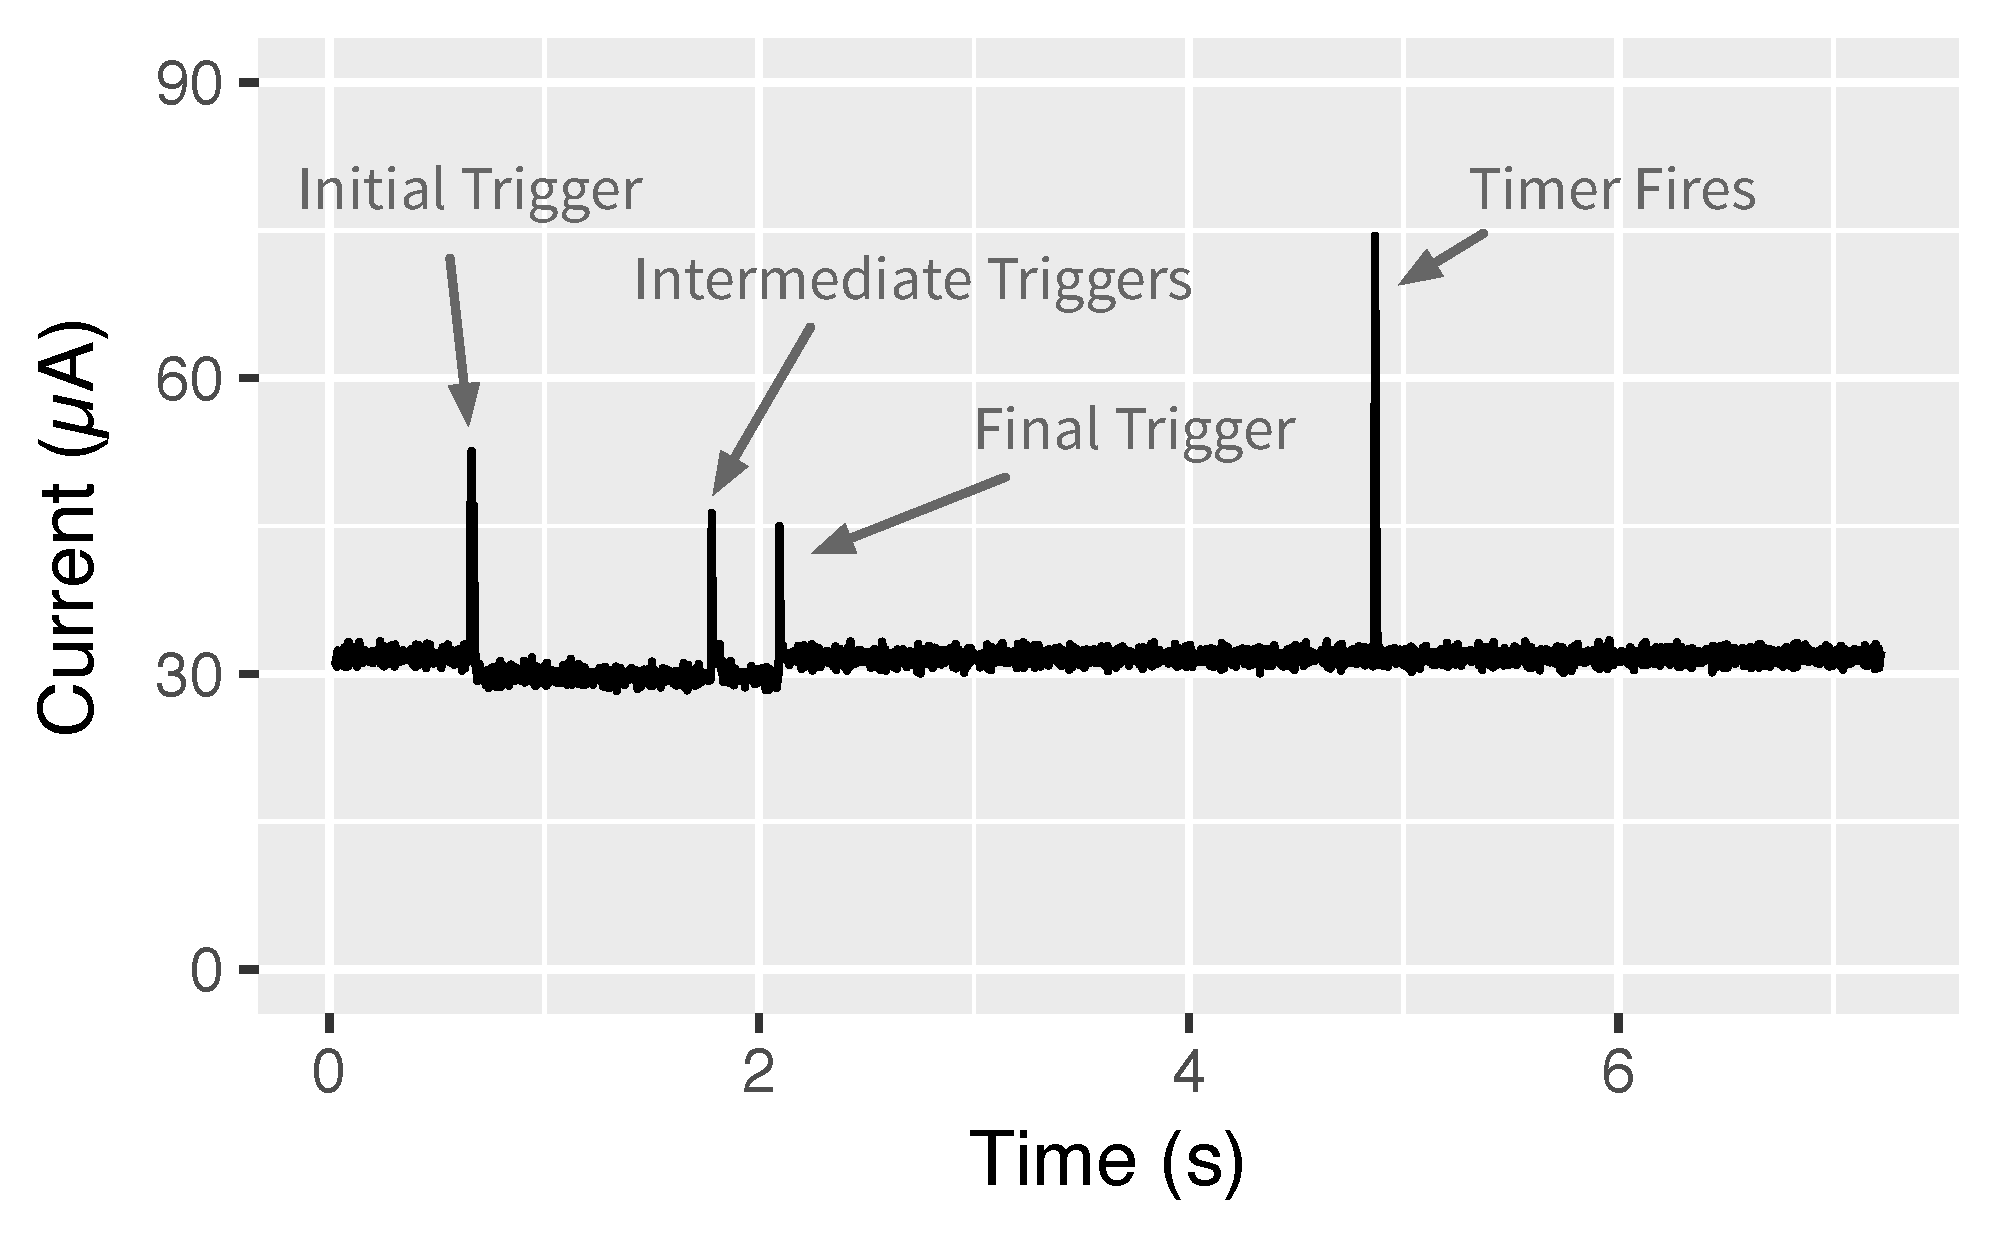
\includegraphics[width=\columnwidth]{figs/profile_final.pdf}
    \caption{ \sysname current draw profile showing differentiators triggering and subsequent current draw spikes during active mode processing by MCU.}
    \label{fig:currentprofile}
\end{figure}

\begin{table}[t]
	\begin{tabular}{@{}p{1.3in}p{0.8in}p{0.8in}@{}}
	\toprule
	\textbf{Event/State} & \textbf{Current} & \textbf{Duration} \\ \midrule
	Idle & 30uA & N/A \\
	Port Interrupt & 60uA & 4ms \\
	Timer Interrupt & 90uA & 8ms \\
	Power On Reset & 300uA & 50ms \\
	\bottomrule
	\end{tabular}
	\caption{\sysname microbenchmarks showing current draw and duration of system level events. When not in power failure, idle current is the passive draw of the differentiator detector circuits.  \label{tab:microbench}}
\end{table}



%\fxnote{[ I created  confusion matrix using R based on the collected data, but that data needs some cleaning like i+o, (i+)o in the %detected direction-AA]}
%section:  System Accuracy
	%just walking through
		%-just using interrupts
		%-just detection circuits
		%hw detection only vs sw enhancements
	%detecting direction
		%-just using interrupts
		%-just detection circuits
		%hw detection only vs sw enhancements
%if we get to sw at all





%section:  extreme cases (how low can we make lighting and system still work)?
